\documentclass[10pt]{article}
\usepackage{icmlko}

\icmlmeta{IP 파운데이션 월드모델}{350}{되돌림은 안 되고 빼기는 된다}{노트 349의 교훈을 위키에 적용했다 --- 둘에서는 안 보이던 것이 넷에서 보인다}

\begin{document}

\twocolumn[
\icmlheader

\begin{abstract}
노트 349가 달력을 아홉 도메인에서 빼 판 $+$0.0044(11/12)를 얻고 둘을
남겼다 --- ① 애니에 달력을 되돌릴까(빼니 $-$0.0075였다) ② 위키를 다시
크게 빼 볼까. \textbf{둘을 한 실험에 넣었다.}

\begin{center}\footnotesize
\begin{tabular}{lrrl}
\hline
처치 & 판 & 양수 & \\
\hline
B 달력을 애니에 되돌림 & $-$0.0005 & 5/12 & \textbf{0} \\
\textbf{C$-$B 위키를 넷에서 뺌} & \textbf{$+$0.0033} & \textbf{10/12} & \\
\hline
\end{tabular}
\end{center}

\textbf{되돌림은 0 이다.} 노트 349에서 애니가 달력을 잃고 $-$0.0075 였는데,
\textbf{돌려줘도 안 돌아온다.} 판이 그 사이 바뀌었고 애니는 이미 다른
축으로 그 자리를 메웠다.

\textbf{빼기는 된다.} 노트 342의 지도에서 위키가 양수 3/8 이하인 넷 ---
웹툰 · 팝업 · 애니 · 시장팝업 --- 에서 뺐다. \textbf{시장팝업이
$+$0.0557(10/12)} 오른다. 지도가 $-$0.0873(0/8)이라 적은 바로 그 자리다.

\textbf{노트 349의 교훈이 두 번째로 맞았다.}

\begin{center}\small
\begin{tabular}{lrrr}
\hline
 & 칸 & 판 & 양수 \\
\hline
위키 둘(노트 341) & 6 & $+$0.0009 & 7/12 \\
\textbf{위키 넷}(오늘) & 12 & \textbf{$+$0.0033} & \textbf{10/12} \\
달력 아홉(노트 349) & 54 & $+$0.0044 & 11/12 \\
\hline
\end{tabular}
\end{center}

\textbf{같은 종류의 처치가 칸 수를 따라 커진다.} 노트 341이 ``빼기는 값이
없다''로 읽은 것은 여섯 칸이었기 때문이다.

챔피언에 위키 컷만 넣었다(달력은 둘 그대로). \textbf{판 0.4859 $\to$
0.4931} --- 아이돌 0.4862 · 시장팝업 0.2823.
\end{abstract}
]

\section{되돌림은 0}

\begin{figure*}[t]
\centering
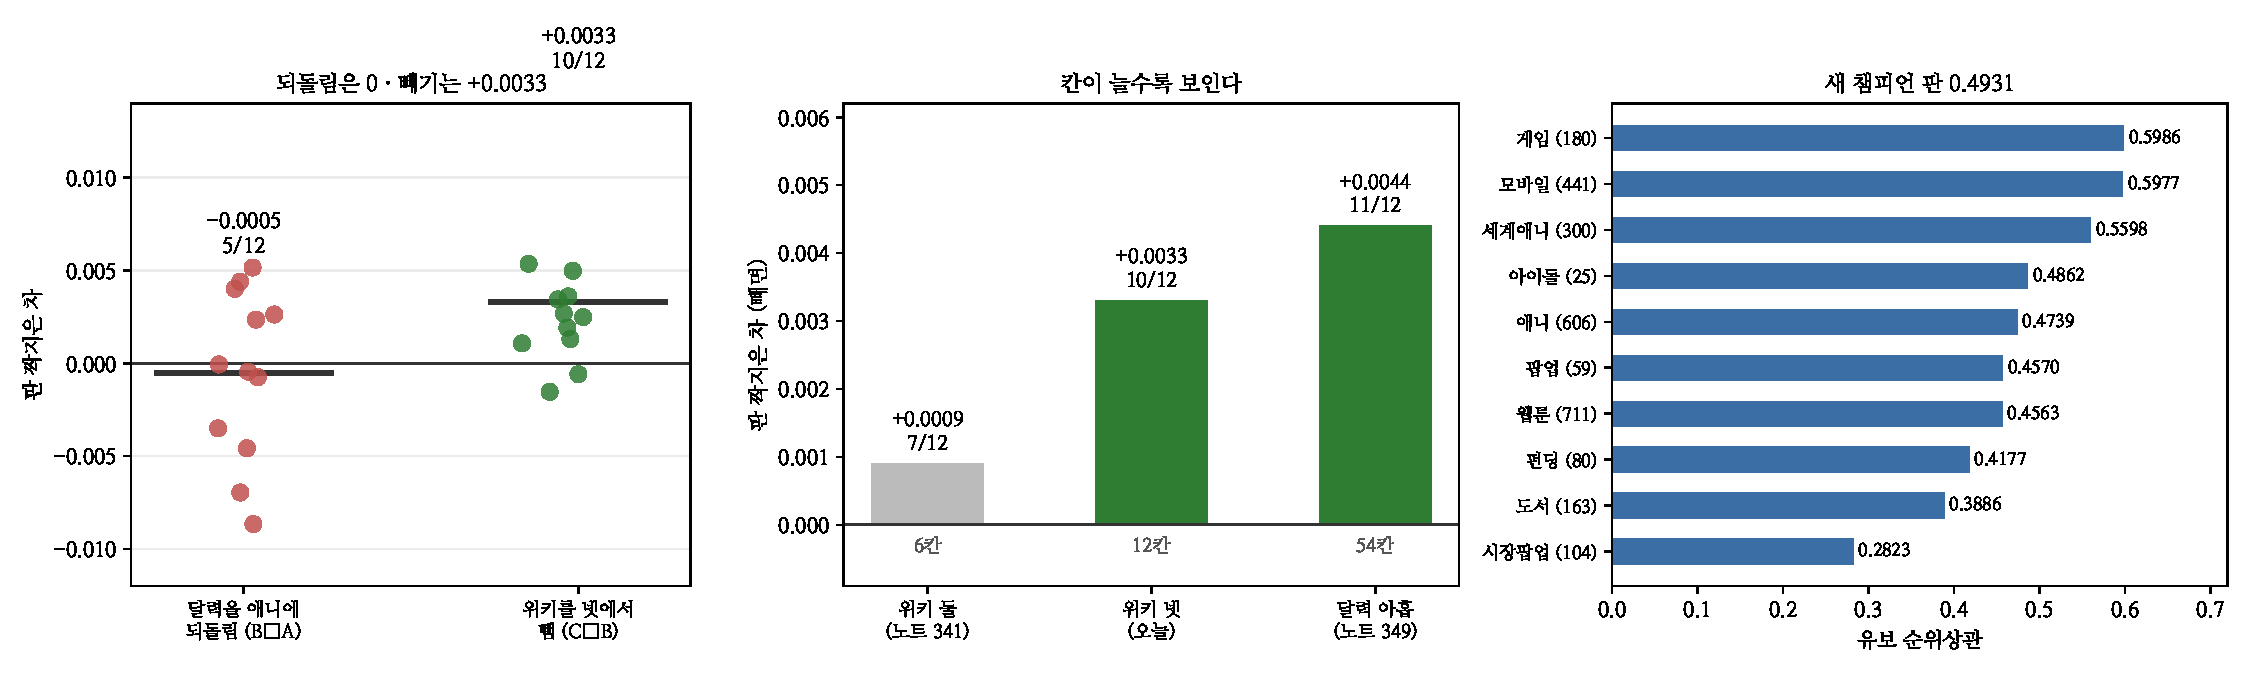
\includegraphics[width=\textwidth]{figs/bigcut.pdf}
\caption{왼쪽 --- 두 처치. 가운데 --- 빼기의 규모 셋. 오른쪽 --- 새 챔피언.}
\end{figure*}

노트 349에서 달력을 아홉에서 빼자 애니만 $-$0.0075(2/12)였다. 지도가
애니를 $+$0.0072(5/8) ``못 가른다''로 적었는데 빼니 손해가 났으니,
\textbf{되돌리면 회복될 것}이라고 봤다. \textbf{$-$0.0005(5/12) 다.}

\textbf{판은 그새 바뀌었다.} 노트 349에서 달력을 뺀 뒤로 애니는 태그 ·
검색 · 위키로 예측을 다시 짰고, 달력을 돌려주면 \emph{또 하나의 열}일
뿐이다. \textbf{뺀 것을 되돌리는 것은 안 뺀 것과 다르다.}

\section{빼기는 칸 수를 따른다}

\begin{center}\footnotesize
\begin{tabular}{lrrrr}
\hline
처치 & 도메인 & 축 & 칸 & 판 \\
\hline
위키(341) & 2 & 3 & 6 & $+$0.0009 (7/12) \\
\textbf{위키(350)} & 4 & 3 & \textbf{12} & \textbf{$+$0.0033 (10/12)} \\
달력(349) & 9 & 6 & 54 & $+$0.0044 (11/12) \\
\hline
\end{tabular}
\end{center}

\textbf{여섯 칸에서는 안 보이고 열두 칸에서 보인다.} 판 짝지은 SD 가
0.004 쯤이니 $+$0.0009 는 0.2$\sigma$ 이고 $+$0.0033 은 0.8$\sigma$ 다 ---
\textbf{효과가 없었던 게 아니라 자보다 작았다.}

\section{시장팝업이 되돌아온다}

\begin{center}\footnotesize
\begin{tabular}{lrrl}
\hline
도메인 & 차(C$-$A) & 양수 & 지도(342) \\
\hline
\textbf{시장팝업} & \textbf{$+$0.0557} & 10/12 & $-$0.0873 (0/8) \\
펀딩 & $+$0.0134 & 8/12 & $+$0.0035 \\
애니 & $+$0.0103 & 10/12 & $-$0.0070 (0/8) \\
세계애니 & $+$0.0056 & 10/12 & $+$0.0584 \\
도서 & $-$0.0214 & 3/12 & $-$0.0017 \\
아이돌 & $-$0.0710 & 1/12 & $-$0.0044 \\
\hline
\end{tabular}
\end{center}

\textbf{지도가 0/8 로 적은 둘(시장팝업 · 애니)이 뺀 뒤에 오른다.}
검사 ⑤ 가 도메인 수준에서 옳았다.

\paragraph{아이돌 $-$0.0710 은 달력 탓이다} C 는 달력 되돌림과 위키 컷을
같이 넣은 팔이다. 위키 컷만 넣어 챔피언을 다시 재니 \textbf{아이돌이
0.4862} 로 오히려 높다 --- \textbf{$-$0.0710 은 B 가 만든 것이었다.}
그래서 최종 챔피언에는 \textbf{위키 컷만} 넣었다.

\section{새 챔피언}

\begin{center}\footnotesize
\begin{tabular}{lr|lr}
\hline
게임 & 0.5986 & 팝업 & 0.4570 \\
모바일 & 0.5977 & 웹툰 & 0.4563 \\
세계애니 & 0.5598 & 펀딩 & 0.4177 \\
아이돌 & 0.4862 & 도서 & 0.3886 \\
애니 & 0.4739 & 시장팝업 & 0.2823 \\
\hline
\multicolumn{4}{c}{\textbf{판 0.4931}} \\
\hline
\end{tabular}
\end{center}

\section{남은 것}
\begin{center}\footnotesize
\begin{tabular}{ll}
\hline
갈래 & 왜 \\
\hline
\textbf{지도를 다시 그려라} & 노트 342 이후 판이 여덟 번 바뀌었다 \\
검색도 크게 빼 볼까 & 지금은 팝업 하나만 진다 \\
태그의 진 자리 & 도메인 전용이라 뺄 게 없다 \\
도서가 왜 $-$0.0214 인가 & 위키를 안 뺐는데 내려간다 \\
\hline
\end{tabular}
\end{center}

\paragraph{규약} \textbf{되돌리기는 안 하기와 다르다.} 노트 349가 애니에서
달력을 빼 손해를 봤고, 그러면 돌려주면 될 것 같다. \textbf{안 된다} ---
그 사이 모형이 다시 짜였고 돌려준 열은 새 열이다. \textbf{그래서 ``빼서
손해면 되돌린다''는 규칙은 이 판에서 안 통한다.} 손해가 났으면
\emph{그 도메인에서 다른 것을 주는} 쪽이 맞고, 그것이 무엇인지는
지도를 다시 그려야 안다.

\end{document}
